\section{Results}\label{sec:results}

\subsection{The filing is legible (H1)}\label{sec:gate1}

Table~\ref{tab:gate1}, Panel A, is the ladder of nested models. On the \NGateOne{} clean-label divisions a cross-validated logistic model on the filing's financial covariates orders disposed from retained subsidiaries with an AUC of \NestedMZero{}, no better than chance in 2001--2016 (\NestedMZeroOld{}). Adding the seven stated-purpose categories that a hand coder would record, the categories \citeA{kang2025} used, raises it to \NestedMOne{} (increment \NestedIncMOneMZero{}); adding the five mention flags---buyer, outside investor, listing, protection measures, appraisal right---adds little more (\NestedMTwo{}). Adding the disposal signal raises the model to \NestedMThree{}, an increment of \NestedIncMThreeMTwo{} with a paired-bootstrap interval of [\NestedIncMThreeMTwoLo, \NestedIncMThreeMTwoHi] and a likelihood-ratio $p$ \NestedLRpMThree{}; the signal alone reaches \NestedS{}, and keyword flags read from the raw text without any model add \NestedIncKOneMZero{} to the financial baseline. The holistic reading is therefore not a finer version of the purpose code: the facts a coder extracts explain \DecompRTwo{} of the variance of $S$---the sale-purpose category alone moves it by \DecompSaleCoef{} and fund-raising by \DecompFundCoef{}---and the residual, what the models read beyond those facts, orders the outcomes with an AUC of \DecompAUCResid{} on its own. Permuting the labels returns mean cross-validated AUCs between \PermAUCMin{} and \PermAUCMax{} for every model. The content that carries the information is the counterparty-addressed statement the disclosure strand predicts: Doosan's 2021 filing stated that the parent would sell its entire stake in the new company to an affiliate (signal \ExDoosanScore{}; \ExDoosanOutcome{}); CJ ENM's 2020 filing listed ``attracting outside investment \ldots{} and the sale of shares where necessary'' among its purposes (\ExTvingScore{}; \ExTvingOutcome{}); DB HiTek's 2023 filing wrote a shareholder vote before any listing into both companies' charters (\ExDBScore{}; \ExDBOutcome{}).

\begin{table}[htbp]
\centering
\caption{The filing predicts the disposal: nested models and the hazard of disposal}\label{tab:gate1}
{\footnotesize\singlespacing\setlength{\tabcolsep}{3pt}
\emph{Panel A. Cross-validated AUC of nested disposal models}\par\smallskip
% generated by code/make_tables_jifma.py on 2026-11-14 — source: results/nested_models_20261110.json -> ladder_pooled, ladder_by_period, increments
\begin{tabular}{l>{\raggedright\arraybackslash}p{6.0cm}cccrr}
\toprule
Model & Inputs & CV AUC & Brier & $\Delta$AUC [95\% CI] & 2001--2016 & 2017+ \\
\midrule
M0 & Financial covariates of the filing & 0.587 & 0.209 & -- & 0.445 & 0.581 \\
M1 & M0 + stated-purpose categories (Kang--Lee type) & 0.667 & 0.200 & +0.080 [0.044, 0.115] & 0.566 & 0.668 \\
M2 & M1 + mention flags (buyer, investor, listing, protection, appraisal) & 0.680 & 0.198 & +0.013 [$-$0.014, 0.039] & 0.599 & 0.733 \\
M3 & M2 + disposal signal $S$ & 0.770 & 0.170 & +0.091 [0.052, 0.128] & 0.706 & 0.830 \\
F & Extracted facts only (purpose + mentions) & 0.611 & 0.205 & -- & 0.593 & 0.689 \\
K1 & M0 + keyword flags read from the raw text, no model & 0.590 & 0.210 & +0.003 [$-$0.026, 0.028] & 0.521 & 0.600 \\
S & Signal alone & 0.758 & 0.172 & -- & 0.700 & 0.809 \\
\bottomrule
\end{tabular}
\par\medskip
\emph{Panel B. Cox model of the time from division to first disposal}\par\smallskip
% generated by code/make_tables_jifma.py on 2026-11-14 — source: results/cox_time_to_disposal_20261110.json -> models.A.cox_strata_period, kaplan_meier_sample_A, expectation_check.HR_S_per_sd
\begin{tabular}{lcccc}
\toprule
 & HR & 95\% CI & $p$ & \\
\midrule
Disposal signal $S$, per standard deviation & 1.96 & [1.74, 2.19] & $<$0.001 & \\
Controlling block, per 10 pp & 0.964 & [0.908, 1.024] & 0.232 & \\
Relative size of the new company & 4.54 & [1.23, 16.75] & 0.023 & \\
Parent leverage after the division & 2.70 & [1.28, 5.70] & 0.009 & \\
log new-company assets & 0.852 & [0.772, 0.941] & 0.002 & \\
KOSDAQ parent & 1.001 & [0.775, 1.292] & 0.993 & \\
\midrule
Kaplan--Meier share disposed by signal tercile & by year 1 & by year 3 & by year 5 & $n$ \\
\midrule
Low $S$ (0.13--0.44) & 24\% & 33\% & 39\% & 163 \\
Middle (0.44--0.57) & 54\% & 74\% & 82\% & 160 \\
High $S$ (0.57--0.99) & 74\% & 83\% & 85\% & 161 \\
\bottomrule
\end{tabular}
}
\tabnote{Panel A: logistic models of the clean-label disposal indicator on the \NGateOne{} divisions, estimated with repeated stratified five-fold cross-validation (50 repeats); M0 uses the characteristics stated in the filing (new company's assets, debt to assets and sales to assets; relative size; surviving company's debt to assets; listing application; put-option contract; market). Purpose categories and mention flags are the majority vote of the models' structured extractions; keyword flags are regular-expression matches on the raw text. $\Delta$AUC is the paired-bootstrap increment over the preceding row (K1 over M0). Panel B: Cox proportional-hazards model stratified by period (2001--08, 2009--16, 2017+) on \CoxN{} divisions with a recorded disposal year (\CoxEvents{} disposals; concordance \CoxConcordance{}); time is the fiscal year of the first ownership change, censored at the latest report. The hazard ratio of $S$ per standard deviation is the per-unit ratio raised to the sample standard deviation of $S$. Kaplan--Meier shares are the cumulative proportion disposed of by the end of the stated fiscal year after the division.}
\end{table}

Panel B treats the censoring of young labels directly. In a Cox model of the time from division to first disposal, stratified by period and conditional on the filing controls and the block, the hazard of disposal rises by a factor of \CoxHRSD{} per standard deviation of the signal (95 percent interval \CoxHRSDLo--\CoxHRSDHi); a permuted signal returns a ratio of \CoxPermHR{} with an interval covering one, and a synthetic sample with a known ratio recovers it. The Kaplan--Meier shares in Panel B (drawn in Figure S1) put the ratio in shares: within one fiscal year of the division \KMLowOneY{} percent of the subsidiaries in the lowest tercile of the signal had changed hands, against \KMMidOneY{} in the middle and \KMHighOneY{} in the top tercile; the baseline hazard is front-loaded (\KMAllOneY{} percent of all subsidiaries within a year, \KMAllFiveY{} within five), so the first year after a division is when the controller's intention is executed, and the filing is sharpest about exactly those disposals (AUC \AUCEarlyPooled{} for disposals within a year against the retained, \AUCLateVsNever{} for disposals two or more years later). The controlling block, conditional on the signal, has a hazard ratio of \CoxHRBlock{} per ten percentage points (\CoxHRBlockLo--\CoxHRBlockHi): what the block tells us about the disposal is already in the filing, the chain H2 predicts.


\subsection{The market's reaction and the year after (H3)}\label{sec:market}

The announcement reaction does not fall with the disposal signal; it rises. With year fixed effects the slope of the three-day abnormal return on the signal is \AnnCarSlope{} ($p$ = \AnnCarSlopeP{}), so a filing that reads as a certain disposal is received \AnnCarSlopePP{} percentage points more favourably than one that reads as a certain retention (Table~\ref{tab:returns}, Panel B); the slope is \AnnSSector{} with GICS-sector effects and parent-clustered errors ($p$ = \AnnSSectorP{}) and \AnnSPlusPurposeMentions{} once the purpose and mention dummies are added ($p$ = \AnnSPlusPurposeMentionsP{}), so the favourable reception attaches to the stated growth story rather than to the residual reading. The return over the following year falls with the signal. The Spearman correlation between the signal and the one-year market-adjusted return is \SpearmanScoreBhar{} across \NScoreOneY{} parents ($p$ = \SpearmanScoreBharP{}); the median return in the top quintile of the signal is \QFiveMedian{} percent against \QOneMedian{} in the bottom quintile (Figure~\ref{fig:signal}). Panel A of Table~\ref{tab:returns} carries the within-year rank of the return across specifications. The coefficient on the signal is \RankSpecThreeCoef{} with year effects, HC1 errors and the full controls, which places a filing at the disposal end of the signal \RankSpecThreePctl{} percentiles lower in its year's ranking than one at the retention end; it is \RankSSector{} with year and GICS-sector effects and parent-clustered errors ($p$ = \RankSSectorPFirm{}; \RankSSectorPTwoway{} with two-way clustering), \RankSPlusPurposeMentions{} with the purpose and mention dummies added ($p$ = \RankSPlusPurposeMentionsP{})---the drift attaches to the reading, not to the categories---and \RankSForeign{} with foreign ownership added ($p$ = \RankSForeignP{}; foreign ownership itself is unrelated to the rank). On the 2015+ subsample with the outside-director ratio the coefficient is \RankSBoard{} ($n$ = \RankSBoardN{}, $p$ = \RankSBoardP{}), imprecise rather than smaller.

\begin{table}[htbp]
\centering
\caption{Returns on the disposal signal: specifications and benchmarks}\label{tab:returns}
{\footnotesize\singlespacing\setlength{\tabcolsep}{3pt}
% generated by code/make_tables_jifma.py on 2026-11-11 — source: results/industry_fe_firm_clusters_20261110.json -> table6_returns_on_signal; nested_models_20261110.json -> return_ladder; governance_controls_20261110.json -> regressions
\begin{tabular}{l>{\raggedright\arraybackslash}p{7.2cm}ccr}
\toprule
 & Specification & Coefficient on $S$ (s.e.) & $p$ & $n$ \\
\midrule
\multicolumn{5}{l}{\emph{Panel A. Within-year rank of the one-year market-adjusted BHAR}} \\
(1) & Year FE, HC1 & $-$0.195 (0.068) & 0.004 & 559 \\
(2) & Year + GICS sector FE, firm cluster & $-$0.194 (0.067) & 0.004 & 559 \\
(3) & Year + GICS sector FE, two-way cluster & $-$0.194 (0.046) & $<$0.001 & 559 \\
(4) & (1) + Kang--Lee-type purpose and mention dummies & $-$0.296 (0.085) & $<$0.001 & 559 \\
(5) & (1) + foreign ownership & $-$0.211 (0.069) & 0.002 & 540 \\
(6) & (1) + foreign ownership + outside-director ratio (FY2015+) & $-$0.187 (0.121) & 0.119 & 194 \\
\midrule
\multicolumn{5}{l}{\emph{Panel B. Three-day announcement CAR}} \\
(7) & Year FE, HC1 & 0.039 (0.019) & 0.041 & 560 \\
(8) & Year + GICS sector FE, firm cluster & 0.045 (0.019) & 0.020 & 560 \\
(9) & (7) + Kang--Lee-type purpose and mention dummies & 0.037 (0.024) & 0.121 & 560 \\
(10) & (7) + foreign ownership & 0.041 (0.020) & 0.044 & 546 \\
\bottomrule
\end{tabular}
\par\medskip
\emph{Panel C. One-year returns against alternative benchmarks}\par\smallskip
{\scriptsize% generated by code/make_tables_jifma.py on 2026-11-11 — source: results/matched_benchmark_selection_20261110.json -> by_benchmark
\begin{tabular}{>{\raggedright\arraybackslash}p{4.6cm}rcccc}
\toprule
Benchmark & $n$ & Mean BHAR, \% [95\% CI] & Spearman($S$) ($p$) & Rank coef.\ on $S$ ($p$) & Early $-$ never, pp ($p$) \\
\midrule
Market-adjusted (paper) & 559 & $-$5.6 [$-$11.1, +0.4] & $-$0.137 (0.001) & $-$0.195 (0.004) & $-$13.6 (0.002) \\
5$\times$5 size/B-M portfolio (size fallback) & 540 & $-$8.2 [$-$13.5, $-$2.3] & $-$0.090 (0.036) & $-$0.147 (0.031) & $-$10.0 (0.069) \\
5$\times$5 strict & 513 & $-$7.7 [$-$13.4, $-$1.5] & $-$0.073 (0.101) & $-$0.117 (0.095) & $-$9.6 (0.118) \\
3$\times$3 size/B-M portfolio & 513 & $-$8.1 [$-$13.8, $-$1.8] & $-$0.085 (0.056) & $-$0.164 (0.019) & $-$8.8 (0.075) \\
Matched firm (size, B/M) & 504 & $-$8.6 [$-$17.6, +0.3] & $-$0.026 (0.555) & $-$0.017 (0.820) & $-$9.4 (0.316) \\
Propensity-matched control firm & 522 & $-$3.6 [$-$11.2, +3.7] & $-$0.088 (0.045) & $-$0.124 (0.071) & $-$15.1 (0.027) \\
\bottomrule
\end{tabular}
}}
\tabnote{Panels A and B: OLS coefficient on the disposal signal (0--1) with the standard error in parentheses. All specifications include announcement-year fixed effects and the controls of Section~\ref{sec:returns} (log market capitalisation, log book-to-market, six-month pre-announcement market-adjusted return, KOSDAQ, relative size of the new company, surviving company's debt to assets, stated listing application; missing values at the median with indicators). (2), (3) and (8) add GICS-sector fixed effects of the parent from Compustat Global; the $p$-value in (2) and (8) uses parent-clustered errors, in (3) two-way parent-and-year clustering; (4) and (9) add the seven purpose-category and five mention dummies of Table~\ref{tab:gate1}; (5), (6) and (10) add foreign ownership at day $-1$ and, in (6), the outside-director ratio. Panel C: the one-year BHAR of the same parents against each benchmark; the rank coefficient is from specification (1) with the within-year rank of the benchmark-adjusted return as dependent variable ($p$ parent-clustered); early $-$ never is the difference in mean BHAR between subsidiaries disposed of within a fiscal year and those retained (Mann--Whitney $p$). The $5\times5$ portfolio falls back to the size quintile when the book-to-market cell is empty; the strict row drops those events.}
\end{table}

Panel C asks whether the drift is the benchmark. Against the parent's $5\times5$ size and book-to-market portfolio the mean one-year abnormal return is \BenchPfSizebmWithSizeFallbackMean{} percent, the rank coefficient on the signal \BenchPfSizebmWithSizeFallbackRank{} ($p$ = \BenchPfSizebmWithSizeFallbackRankP{}) and the Spearman correlation \BenchPfSizebmWithSizeFallbackRho{}; against the $3\times3$ portfolio the coefficient is \BenchPfRank{} ($p$ = \BenchPfRankP{}), and against a propensity-matched control firm \BenchPsmControlFirmRank{} ($p$ = \BenchPsmControlFirmRankP{}). Against a single matched firm the association disappears (\BenchMatchedFirmSizebmRank{}, $p$ = \BenchMatchedFirmSizebmRankP{}); a one-firm benchmark is noisy, but the result depends on the benchmark being a portfolio, and we say so. The loss is realised where the signal said it would be: parents whose subsidiary changed hands within a fiscal year trail those that retained it by \EarlyNeverDiff{} percentage points against the market (Mann--Whitney $p$ = \EarlyNeverMWP{}) and by comparable margins against the portfolios, the coefficient of realised early disposal on the within-year rank is \EarlySector{} with sector effects and parent clusters ($p$ = \EarlySectorP{}), and when early disposal and the signal enter the rank regression together the signal's coefficient falls to \JointScoreCoef{} ($p$ = \JointScoreP{}): the signal's information about the return is the information it carries about the early disposal. The pattern is the limited-attention rival of H3---(a$'$), (b$'$)---and not the efficient reading.

\begin{figure}[htbp]
\centering
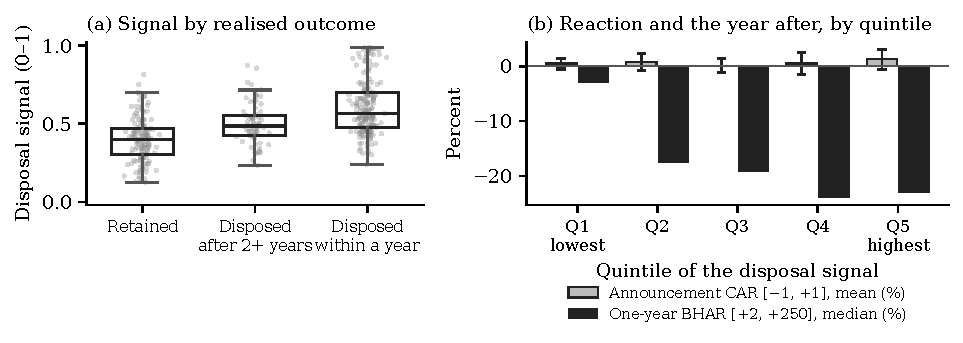
\includegraphics[width=0.86\textwidth]{../figures/F2_signal_outcomes.pdf}
\caption{The disposal signal, realised outcomes and returns}\label{fig:signal}
\tabnote{Panel (a): the two-model disposal signal of the listed parents with a full one-year window, by realised outcome and timing (boxes: interquartile range and median; points: events). Panel (b): mean three-day announcement CAR with bootstrap 95 percent intervals and median one-year market-adjusted BHAR by quintile of the signal.}
\end{figure}

\subsection{The controlling owner's stake (H2 and H3c$'$)}\label{sec:block}

Parents with small controlling blocks wrote the filings that read most as disposals, disposed most often and earned least. In the lowest tercile of the block (up to \LowBlockMax{} percent of common shares) \LowBlockDisp{} percent of subsidiaries were disposed of and \LowBlockEarly{} percent within a year, against \HighBlockDisp{} and \HighBlockEarly{} percent in the top tercile (\HighBlockMin{} percent and above), and the median one-year return was \LowBlockMedian{} against \HighBlockMedian{} percent (Mann--Whitney $p$ \LowHighMWP{}). Table~\ref{tab:block} carries the regressions. The signal falls with the block: \ScoreOnBlock{} per unit of the block with year effects and the controls, \BlockScoreSector{} with sector effects and parent clusters ($p$ = \BlockScoreSectorP{}), \BlockScoreForeign{} with foreign ownership added ($p$ = \BlockScoreForeignP{}; foreign ownership lowers the signal too, \ForeignOnScore{}, $p$ = \ForeignOnScoreP{}) and \BlockScoreBoard{} on the 2015+ subsample with the outside-director ratio ($n$ = \BlockScoreBoardN{}, $p$ = \BlockScoreBoardP{}). The parent's rank in its year's return rises with the block (\RankOnBlock{} per unit, $p$ = \RankOnBlockP{}), and the announcement reaction does not vary with it (\BlockOnCar{}, s.e.\ \BlockOnCarSE{}). The block does not move the hazard once the signal is in the model (Table~\ref{tab:gate1}, Panel B), and in a regression of early disposal on both the block's coefficient is \BlockOnEarlyWithScore{} (s.e.\ \BlockOnEarlyWithScoreSE{}) while the signal's is \ScoreOnEarlyWithBlock{}. The stake works by shaping the intention the filing discloses, which is H2; and the minority holders who bear the loss are those whose controller had the least to lose, which is (c$'$).

\begin{table}[htbp]
\centering
\caption{The controlling block, the signal and the return}\label{tab:block}
{\footnotesize\singlespacing\setlength{\tabcolsep}{3pt}% generated by code/make_tables_jifma.py on 2026-11-14 — source: results/governance_cross_section_20261025.json -> T2; industry_fe_firm_clusters_20261110.json -> table10_block; governance_controls_20261110.json -> block_regressions
\begin{tabular}{l>{\raggedright\arraybackslash}p{6.4cm}ccr}
\toprule
 & Specification & Coefficient on block (s.e.) & $p$ & $n$ \\
\midrule
\multicolumn{5}{l}{\emph{Panel A. Disposal signal $S$ on the controlling block}} \\
(1) & Year FE, controls, HC1 & $-$0.113 (0.045) & 0.013 & 527 \\
(2) & Year + GICS sector FE, firm cluster & $-$0.095 (0.046) & 0.041 & 527 \\
(3) & (1) + foreign ownership & $-$0.143 (0.046) & 0.002 & 508 \\
(4) & (1) + foreign ownership + outside-director ratio (FY2015+) & $-$0.217 (0.093) & 0.018 & 191 \\
\midrule
\multicolumn{5}{l}{\emph{Panel B. Within-year rank of the one-year BHAR on the controlling block}} \\
(5) & Year + GICS sector FE, firm cluster & 0.143 (0.078) & 0.068 & 518 \\
(6) & Year FE + foreign ownership & 0.146 (0.079) & 0.074 & 500 \\
\bottomrule
\end{tabular}
}
\tabnote{OLS coefficient on the controlling block (share, 0--1) with the standard error in parentheses, on the \NOwnership{} listed parents with a pre-announcement ownership record. All specifications include announcement-year fixed effects and the controls of Table~\ref{tab:returns}; (2) and (5) add GICS-sector effects with parent-clustered errors; (3), (4) and (6) add foreign ownership and, in (4), the outside-director ratio (fiscal years from 2014). Panel A's dependent variable is the two-model signal; Panel B's the within-year percentile rank of the one-year market-adjusted BHAR.}
\end{table}

\subsection{The 2022 reform: three channels (H4a--c)}\label{sec:reform}

Table~\ref{tab:reform} takes the reform one channel at a time. \emph{Information (Panel A).} Among 2017--2026 announcements by listed parents, the three-day reaction to a \captive{} rose from \CarCaptivePre{} percent before October 2022 to \CarCaptivePost{} after, while the reaction to an equity spin-off moved from \CarEquityPre{} to \CarEquityPost{} percent. The difference-in-differences with year effects, size and market controls is \DiDCxP{} percentage points (s.e.\ \DiDCxPSE{}, parent-clustered $p$ = \DiDCxPP{}; \DiDNCaptive{} captive and \DiDNEquity{} equity spin-offs, \DiDNPost{} after the cutoff); it is \DiDCxPLong{} on the 2001--2026 sample ($p$ = \DiDCxPLongP{}) and \DiDPlacebo{} ($p$ = \DiDPlaceboP{}) at a placebo cut in October 2019, and the 21-day variant is \DiDCxPTwentyOne{} ($p$ = \DiDCxPTwentyOneP{}), so the gain is concentrated in the announcement window. The filings changed at once: a protection block appears in \ProtPostWithBlock{} of the \ProtPostN{} post-reform filings and in \ProtPreWithBlock{} of \ProtPreN{} earlier ones. What they signal about the disposal did not: the mean signal is \ScorePre{} before and \ScorePost{} after ($p$ = \ScorePrePostP{}), and among divisions old enough to show two years of reports \EarlyPre{} percent disposed within a year before the reform and \EarlyPost{} after (Fisher $p$ = \EarlyPrePostP{}; a comparison that could detect only a change of about \MDEEarlyPP{} points). Relative to the untreated form, the mandate changed what filings say and how they are received, not what they forecast, which is H4a.

\begin{table}[htbp]
\centering
\caption{The 2022 reform through its three channels}\label{tab:reform}
{\footnotesize\singlespacing\setlength{\tabcolsep}{3pt}{\scriptsize% generated by code/make_tables_jifma.py on 2026-11-14 — source: results/equity_did_appraisal_put_20261114.json -> did, appraisal; results/protection_block_20261110.json -> post_by_category, post_tests, coverage
\begin{tabular}{>{\raggedright\arraybackslash}p{6.0cm}rrcc}
\toprule
\multicolumn{5}{l}{\emph{Panel A. Information channel: three-day CAR, captive $\times$ post-October-2022, equity spin-offs as control}} \\
Specification & $n$ (captive / equity) & post & Captive $\times$ post, pp (s.e.) & $p$ \\
\midrule
2017--2026, year FE & 279 (230 / 49) & 65 & 6.72*** (2.19) & 0.002 \\
2017--2026, year FE + log market cap + KOSDAQ & 279 (230 / 49) & 65 & 6.45*** (2.17) & 0.003 \\
2017--2026, 21-day CAR & 260 (211 / 49) & 57 & 3.46 (6.88) & 0.617 \\
2017--2026, CAR winsorised at the 1st/99th percentiles & 279 (230 / 49) & 65 & 5.89*** (1.98) & 0.003 \\
2017--2026, median regression & 279 (230 / 49) & 65 & 3.32* (1.94) & 0.087 \\
2001--2026, year FE + controls & 762 (589 / 173) & 65 & 7.57*** (2.07) & $<$0.001 \\
2001--2026, market-adjusted 3-day return & 762 (589 / 173) & 65 & 7.31*** (2.08) & $<$0.001 \\
Placebo: 2017--Sep 2022 sample, cut at October 2019 & 214 (187 / 27) & 132 & 0.92 (2.04) & 0.658 \\
\midrule
\multicolumn{5}{l}{\emph{Panel B. Deterrence / bonding channel: the shareholder-protection block in post-reform filings}} \\
Category present in the block (a filing may carry several) & Filings & Mean $S$ & Disposed (labelled) & \\
\midrule
Charter / general-meeting special resolution before any listing & 7 & 0.50 & 33\% (6) & \\
No listing for a stated horizon & 3 & 0.34 & 0\% (1) & \\
Sale plan disclosed & 4 & -- & -- (0) & \\
Soft ``remain unlisted'' statement & 32 & 0.45 & 19\% (26) & \\
Payout policy & 3 & 0.62 & 67\% (3) & \\
Disclosure or consultation commitments & 8 & -- & -- & \\
Appraisal right only & 3 & 0.83 & 100\% (2) & \\
Boilerplate, no measure & 15 & 0.68 & 67\% (9) & \\
\multicolumn{5}{l}{61 of the 66 post-reform filings carry a block (75 category mentions); 0 of 228 earlier filings do} \\
\midrule
Strength index of the strongest commitment & Filings & Mean $S$ & Disposed (labelled) & \\
\midrule
3: charter / general-meeting resolution & 7 & 0.50 & 33\% (6) & \\
2: no listing for a stated horizon & 3 & 0.34 & 0\% (1) & \\
1: soft unlisted statement or payout policy & 27 & 0.44 & 17\% (23) & \\
0: no commitment (boilerplate, disclosure, consultation, appraisal only, sale plan) & 29 & 0.66 & 62\% (13) & \\
\multicolumn{5}{l}{Spearman(strength, $S$) $=$ $-$0.27 ($p = 0.075$, $n = 44$)} \\
\midrule
\multicolumn{5}{l}{\emph{Panel C. Compensation channel: the appraisal right as a put}} \\
 & $n$ & & Estimate & $p$ \\
\midrule
Stated appraisal price vs decree formula, median $|$difference$|$ & 26 & & 0.81\% & \\
Moneyness (appraisal price / close$_{-1}$ $-$ 1): median; share in the money & 40 & & 1.55\%; 60\% & \\
Slope of 21-day CAR on moneyness (post-reform captive) & 25 & & 0.45 (0.18) & 0.015 \\
Slope of 3-day CAR on moneyness (post-reform captive) & 33 & & 0.39 (0.28) & 0.172 \\
Placebo: 3-day CAR on formula moneyness, captive 2017--Sep 2022 & 155 & & $-$0.074 (0.041) & 0.072 \\
Placebo: equity spin-offs 2017+ & 20 & & $-$0.165 (0.181) & 0.363 \\
Exercise vs hold one year: median difference, pp; share exercise better & 35 & & 1.09; 51\% & \\
\bottomrule
\end{tabular}
}}
\tabnote{Panel A: OLS of the three-day market-model CAR (percentage points) on a captive indicator, a post-October-2022 indicator (absorbed by year effects where present) and their interaction, on division announcements by listed parents; equity spin-offs are the control; standard errors HC1 in parentheses, $p$-values parent-clustered. Panel B: post-reform \captive{} filings with text, classified by the strongest commitment in the mandatory ``shareholder protection measures'' block; mean two-model signal and share of labelled subsidiaries disposed of. Strength codes 0 (boilerplate or appraisal notice only), 1 (soft statement, payout, disclosure or consultation), 2 (stated no-listing horizon), 3 (charter or general-meeting special resolution). Panel C: the appraisal price stated in the filing relative to the closing price the day before the board resolution; the decree formula (mean of two-month, one-month and one-week volume-weighted average prices) serves as the placebo ratio where no right existed; CAR slopes are OLS with HC1 standard errors. Exercise vs hold compares the stated appraisal price with holding the parent for one year.}
\end{table}

\emph{Compensation (Panel C).} The appraisal price stated in post-reform filings is near the money: median moneyness \MoneynessMedian{} percent (interquartile range \MoneynessQOne{} to \MoneynessQThree{}), in the money for \MoneynessITM{} percent of filings. The 21-day announcement return rises with it, by \PutSlopeTwentyOne{} per percentage point of moneyness ($n$ = \PutSlopeTwentyOneN{}, $p$ = \PutSlopeTwentyOneP{}); the 3-day slope is \PutSlopeThree{} ($p$ = \PutSlopeThreeP{}). The same ratio computed from the formula has a slope of \PutPlaceboPre{} for pre-reform \captive{}s ($p$ = \PutPlaceboPreP{}) and none for equity spin-offs. The right behaves as a put that the market prices, which is H4b; a shareholder who had dissented and exercised would have beaten holding the parent for a year by \ExerciseMinusHold{} percentage points at the median and in \ExerciseBeats{} percent of cases, so the compensation is real and small. \emph{Deterrence and bonding (Panel B).} The presence of the block is uninformative, its content is not. Filings whose strongest commitment is a charter or general-meeting resolution (\ProtCharterVote{} filings), a stated no-listing horizon (\ProtNoListingHorizon{}) or a soft undertaking to stay unlisted (\ProtUnlistedSoft{}) carry mean signals of \ProtMeanSCharter{}, \ProtMeanSHorizon{} and \ProtMeanSUnlisted{}, against \ProtMeanSNone{} for the \ProtNone{} filings that state no measure; the Spearman correlation of commitment strength with the signal is \ProtStrengthRho{} ($p$ = \ProtStrengthP{}), and among labelled subsidiaries \ProtDisposedStrengthZero{} percent of those with no commitment have been disposed of against \ProtDisposedStrengthOne{} percent of those with a soft one ($n$ = \ProtNLabStrengthZero{} and \ProtNLabStrengthOne{}). The \ProtSalePlan{} filings that disclose a sale plan have no labels yet. The content of the block separates intentions in the direction H4c predicts, on a sample too young to carry more than that.
